% Chapter 1
\chapter{Eaglescience}\label{ch:Eaglescience} % Chapter title

Het hier beschreven onderzoek en de daarbij behorende applicatie is uitgevoerd en ontwikkeld in opdracht van het bedrijf Eaglescience. Dit bedrijf is gevestigd in Amsterdam Sloterdijk en houdt zich sinds 2009 bezig met het ontwikkelen van software. Hoewel het ontwikkelen van maatwerk software de kern activiteit is biedt het bedrijf ook een aantal andere diensten aan, zoals het bouwen van prototypes of het meedenken in een designsprint om bedrijven of startups een goede richting te geven voor het ontwikkelen van een project. Daarnaast biedt Eaglescience hosting aan voor de software die zelf is ontwikkeld, om zo garantie te kunnen bieden dat er alles aan wordt gedaan zodat de geleverde software veilig, kwalitatief goed en correct functioneerd.

\section{Organisatie}\label{sec:organisatie}
Eaglescience BV bestaat uit drie divisies: Innovations, Software en Solutions (figuur~\ref{fig:Eaglescience organogram}). Er werken, op het moment van schrijven, $\pm$ 20 medewerkers waarvan 75\% verantwoordelijk is voor de ontwikkeling van software. De andere 25\% bekleed een support rol zoals project manager, finance manager, quality manager, automatisering etc.

\begin{figure}[bth]
\myfloatalign
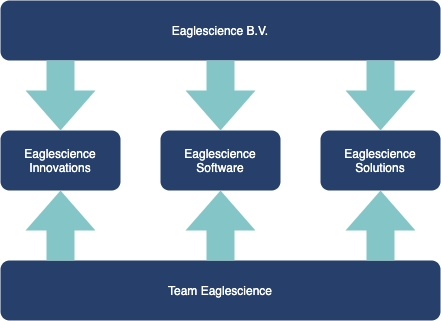
\includegraphics[width=9cm]{gfx/organogram}
\caption{Organogram Eaglescience}
\label{fig:Eaglescience organogram}
\end{figure}
De divisie Eaglescience Innovations zoekt naar nieuwe oplossingen op het gebied van softwareontwikkeling, welke door de divisie Eaglescience Software wordt geïmplementeerd. Eaglescience Solutions onderzoekt en adviseert over oplossingen voor gestelde problemen.

Het dagelijks bestuur is handen van:
\begin{itemize}
\item CEO / CFO - Marc Grootjen
\item CTO - Bas Breier
\item COO - Wender van Mansvelt
\end{itemize}
Onder het dagelijks bestuur valt Team Eaglescience wat bestaat uit projectmanagers en ontwikkelaars. Deze zijn onderverdeeld in diverse scrum teams die ieders verantwoordelijk zijn voor een project. De ontwikkelaars worden parallel ingezet op meerdere projecten om kennisdeling te bevorderen.

\subsection{Missie}\label{subsec:missie}

De missie van Eaglescience is het bedienen van haar partners door een ontwerp, ontwikkeling en service te bieden op het gebied van op maat gemaakte IT-oplossingen. Hiervoor heeft Eaglescience goed opgeleide IT-professionals in dienst die zichzelf continue ontwikkelen op de “cutting edge” van IT-technologie. De hoofdcompetenties van de medewerkers zijn: innovatief, intelligent, klant georiënteerd, flexibel en ambitieus.

\subsection{Visie}\label{subsec:visie}
Eaglescience streeft er als innovatief IT-bedrijf naar om software te ontwikkelen als een Business-to-Business dienst. Middels technische vaardigheden bouwen we veilige en hoogwaardige software die bijdraagt aan een betere wereld. Omdat we Agile werken, leveren we precies wat nodig is, niets meer en niets minder. Wij helpen onze klanten zoeken naar een langdurige betrokkenheid en samenwerking op basis van zowel vertrouwen als wederzijds respect.

Omdat elke vraag uniek is, ontwikkeld Eaglescience op maat gemaakte en innovatieve software.  We zijn van plan deel uit te maken van het hele proces van het formuleren van een idee tot het lanceren van het product en het waarborgen van de productie levenscyclus. Onze belangrijkste succesfactor zijn de mensen, die zich continu ontwikkelen door met de nieuwste technieken te werken op diverse projecten. Wij streven naar een optimale balans tussen werk en privé. Dit geeft onze medewerkers veel vrijheid, maar vereist zelfdiscipline en verantwoordelijkheid.

\subsection{Strategie}\label{subsec:strategie}
Eaglescience levert de visie via vier strategische thema's:
\begin{itemize}
    \item Maatschappelijke verantwoordelijkheid
    \item Persoonlijke groei en werknemer tevredenheid
    \item Kwalitatief hoogstaande producten en diensten
    \item Financieel onafhankelijk en een sociaal verantwoorde groei
\end{itemize}
We streven ernaar om veilige en hoogwaardige software diensten te leveren die waarde toevoegen aan onze samenleving. We streven naar een bedrijfscultuur waarin alle collega's hun talenten kunnen laten groeien. We hebben een ongecompliceerd werkethos: we richten ons op resultaten van hoge kwaliteit, maar met een gezonde balans tussen werk en privé en voldoende tijd voor leuke en sociale evenementen. Eaglescience verwacht van alle medewerkers dat zij hun handelen baseren op vier kwaliteitsprincipes:
\begin{itemize}
    \item Meld situaties die niet voldoen aan onze interne procedures
    \item Evalueer risico's wanneer grote veranderingen worden verwacht
    \item Help en daag elkaar uit
    \item Kennis behouden over compliancy en kwaliteitsmanagement
\end{itemize}

\section{Werkwijze}\label{sec:werkwijze}
Zoals eerder gemeld werkt Eaglescience op projectbasis met ontwikkelaars in meerdere teams. Er wordt geprobeert "full scrum" te werken waarbij de requirements van de klant centraal staan. Als een project wordt aangenomen door het managementteam dan wordt deze in sprints in samenspraak met de klant ontwikkeld. De klant wordt nauw betrokken bij het verloop van de ontwikkeling door het geven van demo's aan het einde van iedere sprint. Hier wordt gemeten hoe de applicatie zich gedraagt met betrekking tot de requirements van de klant. Dit is ook het moment dat er feedback gegeven wordt en waar nodig gestuurd kan worden in het verdere verloop. Op het moment dat er een applicatie klaar is wordt de software al dan niet overgedragen aan de klant of doorgegeven aan support en hosting die verantwoordelijk zijn voor de daadwerkelijke hosting van de software. (figuur~\ref{fig:Project Process})

%TODO: Vertaling checken
\begin{figure}[bth]
\myfloatalign
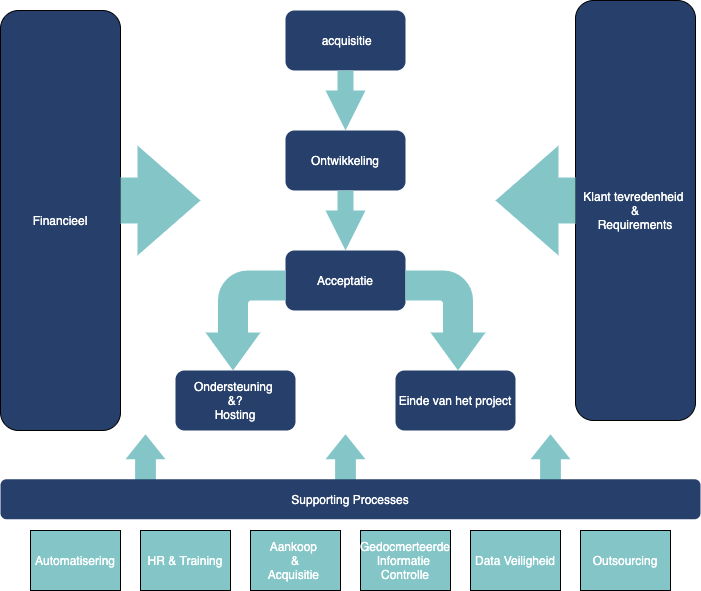
\includegraphics[width=10cm]{gfx/ProcessFlow}
\caption{Project Process}
\label{fig:Project Process}
\end{figure}

Naast het ontwikkelproces zijn er een aantal supporting processen die ervoor zorg dragen dat het bedrijf blijft draaien. Onder deze processen valt ook automatisering die voor ondersteuning zorgt van platformen waarop ontwikkeld en/of gehosted wordt. Eaglescience ontwikkeld en genereerd inkomsten op projectbasis. Alle processen die draaien moeten dus direct ingezet kunnen worden op projecten van klanten. Als er een project voor in huis gebruik wordt ondernomen moet er een duidelijk beeld zijn of er op termijn winst mee te behalen valt op monetair vlak al dan niet tijdswinst of ontwikkelgemak. (figuur~\ref{fig:Project Process})

\section{Relevante en actuele ontwikkelingen binnen Eaglescience}\label{sec:relevante-en-actuele-ontwikkelingen-binnen-Eaglescience}

Eaglescience is aan het groeien, zowel in het aantal projecten waar aan gewerkt wordt als in het aantal medewerkers. Daarnaast worden de diensten die Eaglescience aanbied ook uitgebreid, en wordt het hosten van de ontwikkelde applicaties steeds vaker aangeboden. Door deze inzet ligt de verantwoordelijkheid niet alleen bij het leveren van een veilige en hoogwaardige software, maar ook bij het leveren van een veilige hosting service. Naast de groei van het bedrijf is ook de uitbreiding van diensten die aangeboden worden een reden om taken die geautomatiseerd kunnen worden dan ook te automatiseren.

Daarnaast heeft Eaglescience de afgelopen jaren een portfolio aan verschillende klantproducten opgebouwd. Deze producten worden gehost, onderhouden en er wordt service en support geboden richting gebruikers. Eaglescience is momenteel doende dit onder de noemer Software Lifecycle Management te integreren in het kwaliteitssysteem door middel van beleid en het vastleggen in werkprocessen. Het in de grip en up-to-date houden van de live softwareproducten vraagt om een gerichte-, transparante- en traceerbare aanpak ten aanzien van alle gebruikte software-onderdelen (bibliotheken/ libraries) en onderliggende afhankelijkheden (dependencies).



